\documentclass[12pt]{article}

\usepackage{makeidx}  % allows for indexgeneration
\usepackage{fancyvrb}
\usepackage{setspace}
\usepackage{mdwlist}
\usepackage{multirow} 
\usepackage[pdfborder={0 0 0}]{hyperref}
\usepackage{url}
\usepackage{boxedminipage}
\usepackage{color}
\usepackage{verbatim}
\usepackage{flafter}
\usepackage{listings}
\usepackage{array}
\usepackage{subfig}
\usepackage[figuresright]{rotating}
\usepackage{placeins}
\usepackage{graphicx}
\usepackage[T1]{fontenc}

\title{UH-CAF Performance Test Suite User guide}
\author{Siddhartha Jana, Deepak Eachempati\\
HPCTools Group \\
Department of Computer Science\\
University of Houston, \\
Houston, TX 77204-3010 \\
USA\\
}

\date{17th February, 2013}

\begin{document}
\maketitle

\begin{abstract}
The purpose of this guide is to familiarize users with the UH CAF performance suite, the functionality, and its usage. This guide also enlists some of the initial results of single-node performance of the NPB, built with different CAF implementations, namely - OpenUH (GasNET and ARMCI), Intel(R), and G95.
\end{abstract}

\section{Categories of Tests}
This section outlines the different categories of tests within the suite that can be used to evaluate the performance of binaries generated by a CAF compiler
implementation. 

In this report, ROOT = <parent\_directory of caf\_testsuite> and \$PEFORMANCE\_PATH=<\$ROOT/performance>

There are three main categories of tests in the test suite. Each category is located in a different subdirectory within \$PEFORMANCE\_PATH, and all the tests within the same category can be executed using either the single Makefile in \$PEFORMANCE\_PATH or individual Maefiles within the corresponding subdirectories. 

\subsubsection{Kernels}
These includes some standalone CAF applications. The list includes:
\begin{itemize}
\item CG (2D)
\item Buffon Laplace
\item Image Smoothing
\item Insertion sort
\item Insertion sort (D-type)
\item Matrix Multiplication
\end{itemize}

\subsubsection{Microbenchmarks}
These includes simple CAF codes with point to point communications. The list of test includes:
\begin{itemize}
\item bidirectional
\item get\_bandwidth
\item noncontiguous
\item ping\_pong    
\item put\_latency
\item broadcast
\item get\_latency
\item partial\_data
\item put\_bandwidth
\item Reductions using remote 'get' ops 
\end{itemize}

\subsubsection{NPB}
These include the CAF version of the NAS 3.3.1 The current tests include EP, CG, SP, BT. The EP and CG have been developed at the University of Houston. The SP and BT have been developed by the NAS team @ NASA.




\section{Installation and running the tests}
The performance suite comes bundled along with the validation test suite. The performance suite is located under: 

PERFORMANCE\_PATH = /caf\_testsuite/performance/

The installation requires the setup of a few configuration parameters. These parameters can be divided into two types:
\begin{enumerate}
\item Generic parameters: These are testsuite specific parameters which can be used to specify the location of the compilation, execution result-dumps. These are located in \$PERFORMANCE\_PATH/support/CONFIG
\item Compiler-specific: These are compiler dependent parameters and can be used to adjust the compiler/execution commands, flags and launcher options. These are located in \$PEFORMANCE\_PATH/support/CONFIG-compiler.<compiler>
\end{enumerate}

The configuration parameters are enlisted under section \ref{sec:config}.

\subsubsection{Configuration params}
\label{sec:config}
Table~\ref{tab:params} lists the different options that need to be
set for the test-suite. These options can be initialized in the
CONFIG file in the ``config'' directory. The make.def version of
this file is auto-generated by running the script
config2makedef.sh in the same directory.

\begin{table}[tbh!]
\small
\caption{List of configuration parameters. Here \emph{test\_type}= CONF or FEATURE or FEW or FAULT }
\label{tab:params}
\begin{tabular}{|c|p{6cm}|p{2cm}|}
\hline
Parameter & Description &   Compiler specific(y/n)  \\ \hline
BIN\_PATH   & The path to dump all the executables.  &  NO \\\hline
NPROCS &  Number of images to launch  & NO \\\hline
NITER &  Number of times the test is repeated & NO \\\hline
SLEEP &  This is used to intentionally slow down certain images to cause race conditions while testing certain constructs & NO \\\hline
TIMEOUT & This parameter is passed to the perl script call timedexec.pl which ends processes which exceed the given execution time. This is helpful for backing out while executing tests which deadlock due to incorrect implementation &  NO \\\hline
COMPILER &  compiler name  &  YES \\\hline
FC &  command to invoke the compiler &  YES \\\hline
FFLAGS &  Flags passed to the compiler. The necessary flags include the options to enable the macro preprocessor and define the macros - NPROCS, NITER and SLEEP. &  YES \\\hline
LAUNCHER &  command to launch multiple images  & YES \\\hline
EXEC\_OPTIONS &   Flags passed to the launcher after the executable name. Not so common.  & YES \\\hline
FFLAGS\_CROSS &  Flags passed to the compiler while executing the cross tests. Generally the value include all the options listed for FFLAGS, plus the flag to define the CROSS\_ macro in the tests.  & YES \\\hline
\emph{test\_type}\_COMPILE\_PATH &  Path to dump the messages generated by the compiler.&  NO \\\hline
\emph{test\_type}\_EXEC\_PATH &  Path to dump the output of the executables / the messages generated by the compiler or runtime.&  NO \\\hline
\emph{test\_type}\_TEST\_PATH &  Path to dump the output of the test results.& NO \\\hline
\emph{test\_type}\_LOG\_PATH &  Path to dump the output of the test results.& NO \\\hline
\end{tabular}
\end{table}


\subsubsection{Running the tests}
For running the tests:
\begin{enumerate}
\item cd \$PERFORMANCE\_PATH
\item make [OPTIONS] [COMPILER=uhcaf|ifort|g95] ...
 Where, OPTIONS include:
 \begin{itemize}
 \item <suite>:          [kernels|microbenchmarks|npb|all]
 \item compile\_<suite>: compiles and generates logs for the codes
 \item run\_<suite>:     executes and generates logs for the codes
 \item complete\_<suite>:executes and generates logs for the codes
 \item clean\_<suite>:   cleans up the logs, executables and all previous history of the regression runs
 \item help:             displays this message
 \item cleanall:         cleans up the entire performance test suite
 \end{itemize}
\end{enumerate}




\section{Test results}
This section outlines the performance comparison of the
compilers on a single 4-core machine.

% EP

\begin{figure}[ht]
\begin{minipage}[b]{0.45\linewidth}
\centering
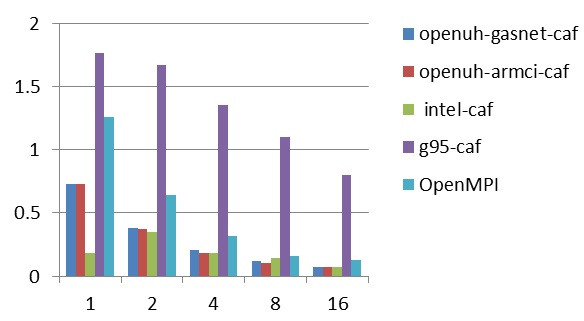
\includegraphics[width=\textwidth]{./figures/ep_S_time.jpg}
\caption{EP, CLASS=S}
\label{fig:figure1}
\end{minipage}
\hspace{0.5cm}
\begin{minipage}[b]{0.45\linewidth}
\centering
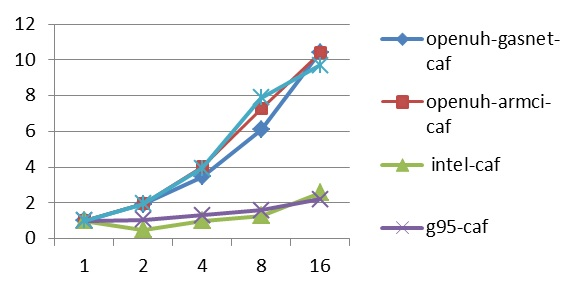
\includegraphics[width=\textwidth]{./figures/ep_S_scalability.jpg}
\caption{EP, CLASS=S}
\label{fig:figure2}
\end{minipage}
\end{figure}


\begin{figure}[ht]
\begin{minipage}[b]{0.45\linewidth}
\centering
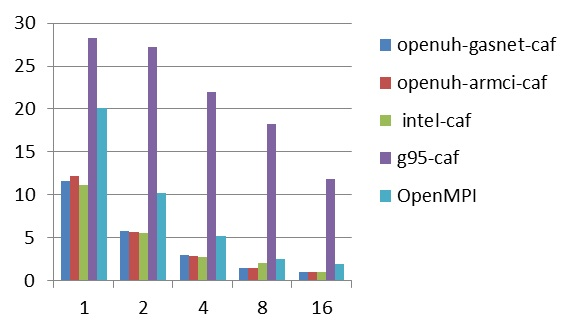
\includegraphics[width=\textwidth]{./figures/ep_A_time.jpg}
\caption{EP, CLASS=A}
\label{fig:figure1}
\end{minipage}
\hspace{0.5cm}
\begin{minipage}[b]{0.45\linewidth}
\centering
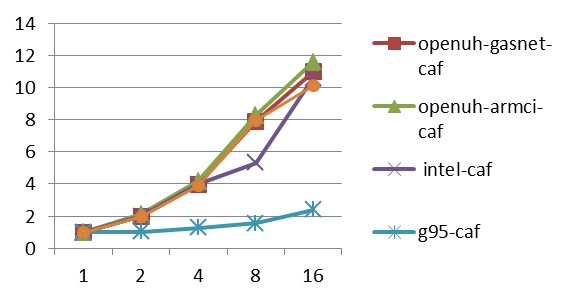
\includegraphics[width=\textwidth]{./figures/ep_A_scalability.jpg}
\caption{EP, CLASS=A}
\label{fig:figure2}
\end{minipage}
\end{figure}



\begin{figure}[ht]
\begin{minipage}[b]{0.45\linewidth}
\centering
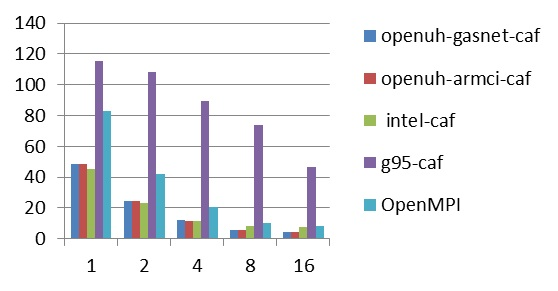
\includegraphics[width=\textwidth]{./figures/ep_B_time.jpg}
\caption{EP, CLASS=B}
\label{fig:figure1}
\end{minipage}
\hspace{0.5cm}
\begin{minipage}[b]{0.45\linewidth}
\centering
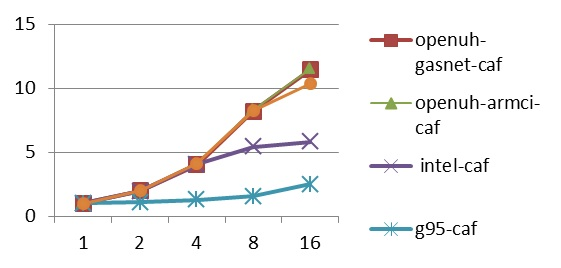
\includegraphics[width=\textwidth]{./figures/ep_B_scalability.jpg}
\caption{EP, CLASS=B}
\label{fig:figure2}
\end{minipage}
\end{figure}


\begin{figure}[ht]
\begin{minipage}[b]{0.45\linewidth}
\centering
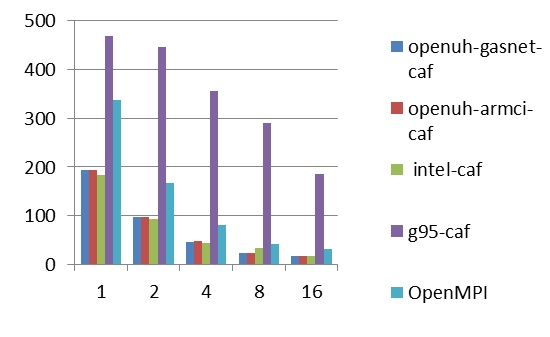
\includegraphics[width=\textwidth]{./figures/ep_C_time.jpg}
\caption{EP, CLASS=C}
\label{fig:figure1}
\end{minipage}
\hspace{0.5cm}
\begin{minipage}[b]{0.45\linewidth}
\centering
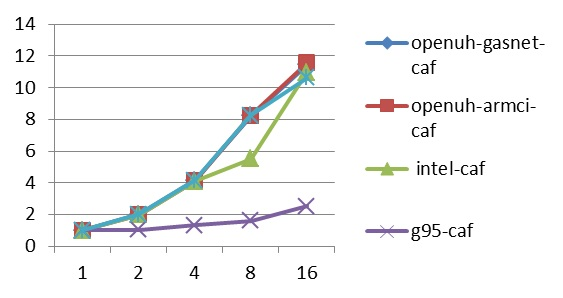
\includegraphics[width=\textwidth]{./figures/ep_C_scalability.jpg}
\caption{EP, CLASS=C}
\label{fig:figure2}
\end{minipage}
\end{figure}



% CG

\begin{figure}[ht]
\begin{minipage}[b]{0.45\linewidth}
\centering
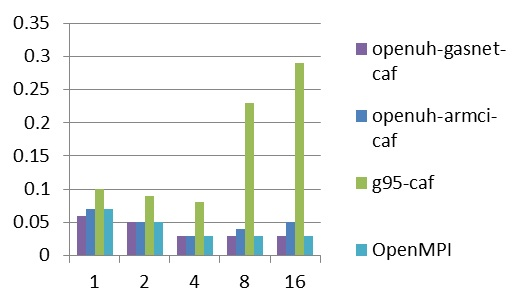
\includegraphics[width=\textwidth]{./figures/cg_S_time.jpg}
\caption{CG, CLASS=S}
\label{fig:figure1}
\end{minipage}
\hspace{0.5cm}
\begin{minipage}[b]{0.45\linewidth}
\centering
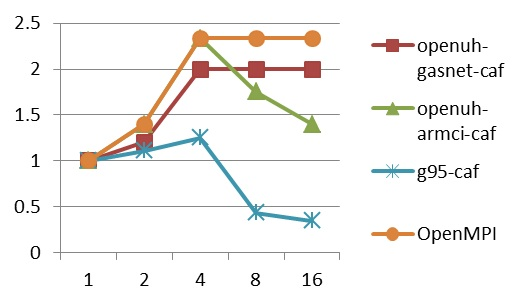
\includegraphics[width=\textwidth]{./figures/cg_S_scalability.jpg}
\caption{CG, CLASS=S}
\label{fig:figure2}
\end{minipage}
\end{figure}


\begin{figure}[ht]
\begin{minipage}[b]{0.45\linewidth}
\centering
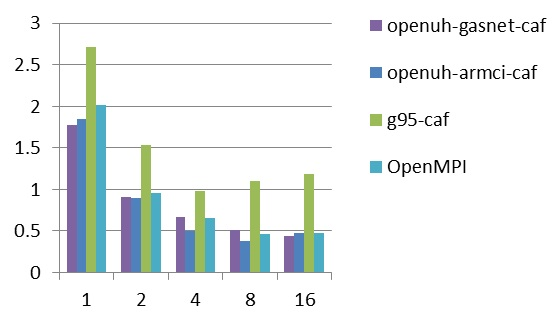
\includegraphics[width=\textwidth]{./figures/cg_A_time.jpg}
\caption{CG, CLASS=A}
\label{fig:figure1}
\end{minipage}
\hspace{0.5cm}
\begin{minipage}[b]{0.45\linewidth}
\centering
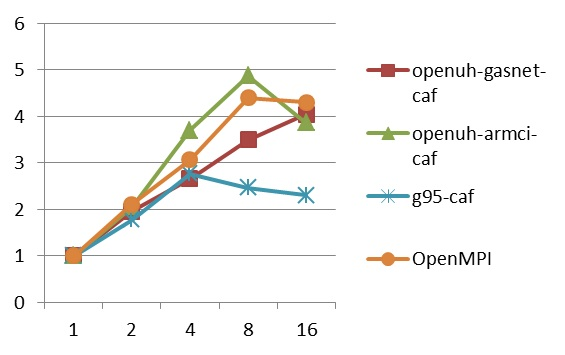
\includegraphics[width=\textwidth]{./figures/cg_A_scalability.jpg}
\caption{CG, CLASS=A}
\label{fig:figure2}
\end{minipage}
\end{figure}



\begin{figure}[ht]
\begin{minipage}[b]{0.45\linewidth}
\centering
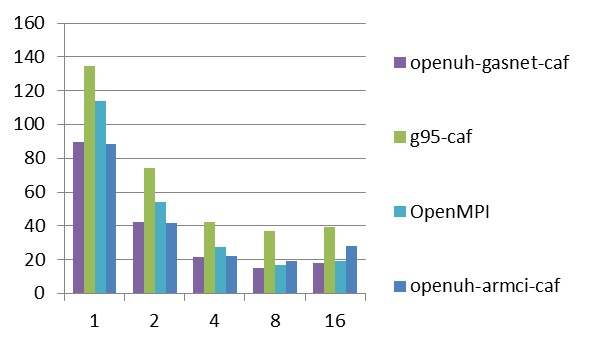
\includegraphics[width=\textwidth]{./figures/cg_B_time.jpg}
\caption{CG, CLASS=B}
\label{fig:figure1}
\end{minipage}
\hspace{0.5cm}
\begin{minipage}[b]{0.45\linewidth}
\centering
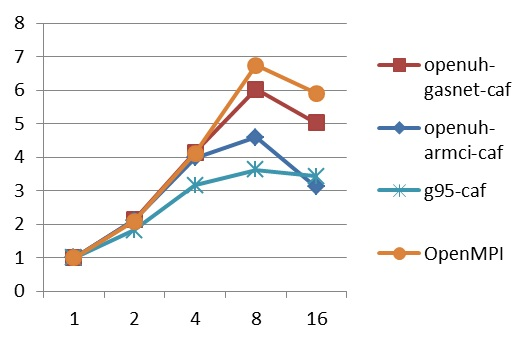
\includegraphics[width=\textwidth]{./figures/cg_B_scalability.jpg}
\caption{CG, CLASS=B}
\label{fig:figure2}
\end{minipage}
\end{figure}


\begin{figure}[ht]
\begin{minipage}[b]{0.45\linewidth}
\centering
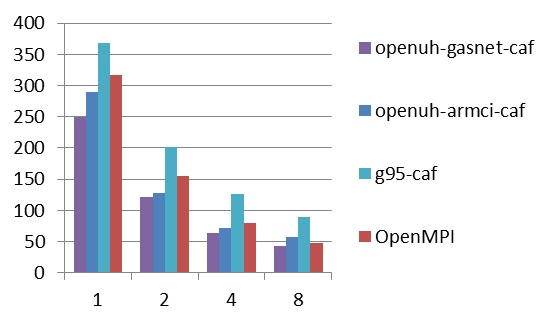
\includegraphics[width=\textwidth]{./figures/cg_C_time.jpg}
\caption{CG, CLASS=C}
\label{fig:figure1}
\end{minipage}
\hspace{0.5cm}
\begin{minipage}[b]{0.45\linewidth}
\centering
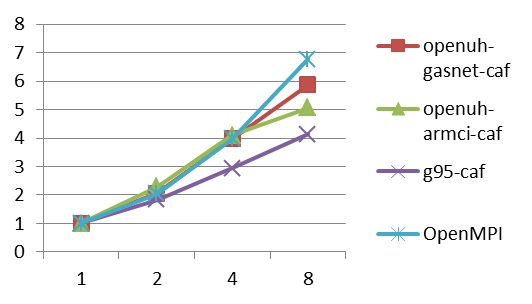
\includegraphics[width=\textwidth]{./figures/cg_C_scalability.jpg}
\caption{CG, CLASS=C}
\label{fig:figure2}
\end{minipage}
\end{figure}

% SP

\begin{figure}[ht]
\begin{minipage}[b]{0.45\linewidth}
\centering
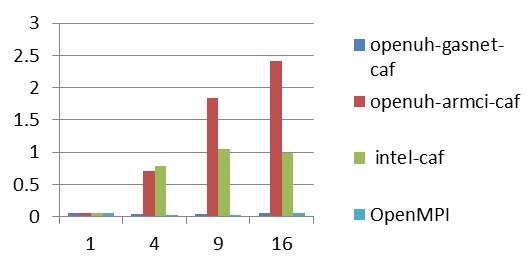
\includegraphics[width=\textwidth]{./figures/sp_S_time.jpg}
\caption{SP, CLASS=S}
\label{fig:figure1}
\end{minipage}
\hspace{0.5cm}
\begin{minipage}[b]{0.45\linewidth}
\centering
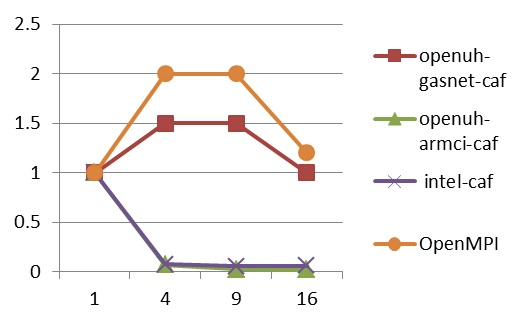
\includegraphics[width=\textwidth]{./figures/sp_S_scalability.jpg}
\caption{SP, CLASS=S}
\label{fig:figure2}
\end{minipage}
\end{figure}


\begin{figure}[ht]
\begin{minipage}[b]{0.45\linewidth}
\centering
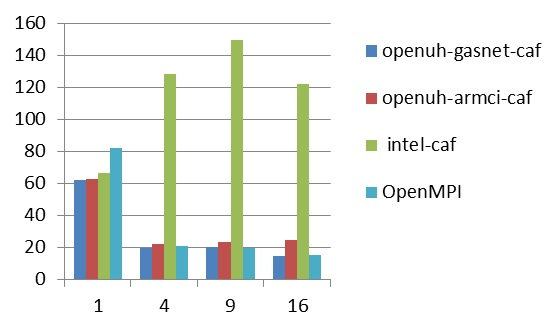
\includegraphics[width=\textwidth]{./figures/sp_A_time.jpg}
\caption{SP, CLASS=A}
\label{fig:figure1}
\end{minipage}
\hspace{0.5cm}
\begin{minipage}[b]{0.45\linewidth}
\centering
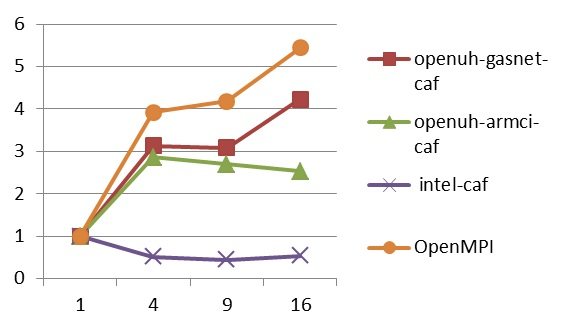
\includegraphics[width=\textwidth]{./figures/sp_A_scalability.jpg}
\caption{SP, CLASS=A}
\label{fig:figure2}
\end{minipage}
\end{figure}



\begin{figure}[ht]
\begin{minipage}[b]{0.45\linewidth}
\centering
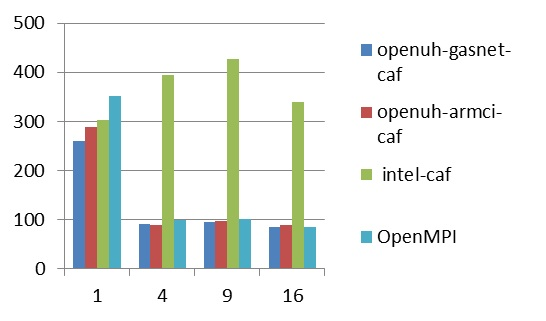
\includegraphics[width=\textwidth]{./figures/sp_B_time.jpg}
\caption{SP, CLASS=B}
\label{fig:figure1}
\end{minipage}
\hspace{0.5cm}
\begin{minipage}[b]{0.45\linewidth}
\centering
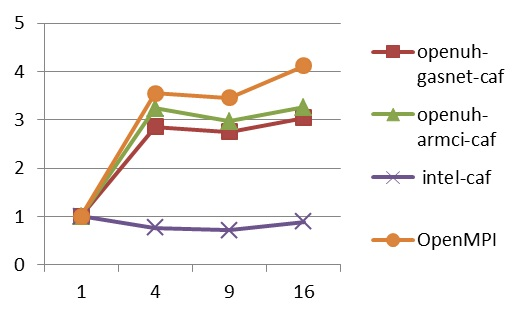
\includegraphics[width=\textwidth]{./figures/sp_B_scalability.jpg}
\caption{SP, CLASS=B}
\label{fig:figure2}
\end{minipage}
\end{figure}


\begin{figure}[ht]
\begin{minipage}[b]{0.45\linewidth}
\centering
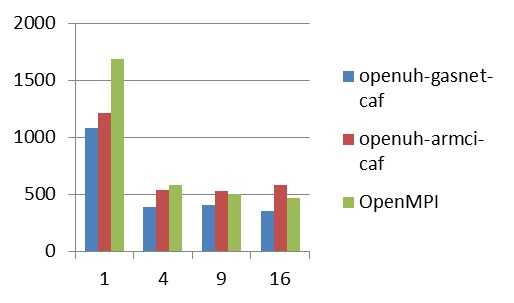
\includegraphics[width=\textwidth]{./figures/sp_C_time.jpg}
\caption{SP, CLASS=C}
\label{fig:figure1}
\end{minipage}
\hspace{0.5cm}
\begin{minipage}[b]{0.45\linewidth}
\centering
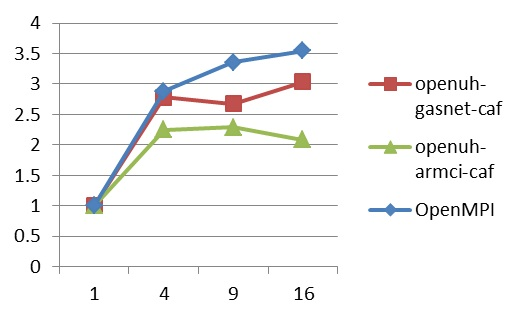
\includegraphics[width=\textwidth]{./figures/sp_C_scalability.jpg}
\caption{SP, CLASS=C}
\label{fig:figure2}
\end{minipage}
\end{figure}

% BT
\begin{figure}[ht]
\begin{minipage}[b]{0.45\linewidth}
\centering
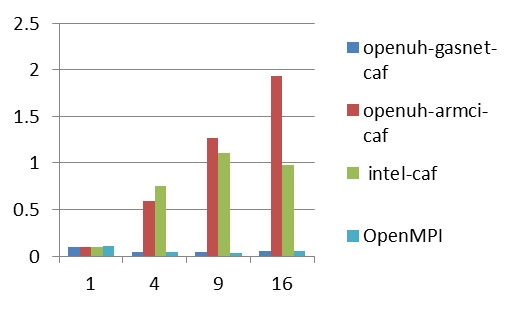
\includegraphics[width=\textwidth]{./figures/bt_S_time.jpg}
\caption{BT, CLASS=S}
\label{fig:figure1}
\end{minipage}
\hspace{0.5cm}
\begin{minipage}[b]{0.45\linewidth}
\centering
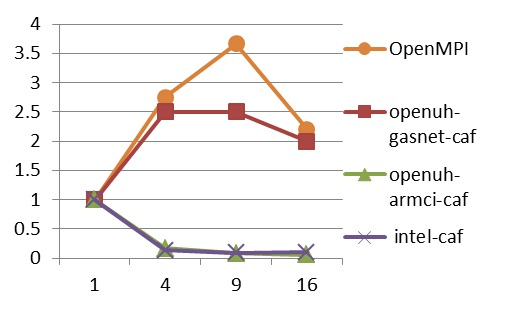
\includegraphics[width=\textwidth]{./figures/bt_S_scalability.jpg}
\caption{BT, CLASS=S}
\label{fig:figure2}
\end{minipage}
\end{figure}


\begin{figure}[ht]
\begin{minipage}[b]{0.45\linewidth}
\centering
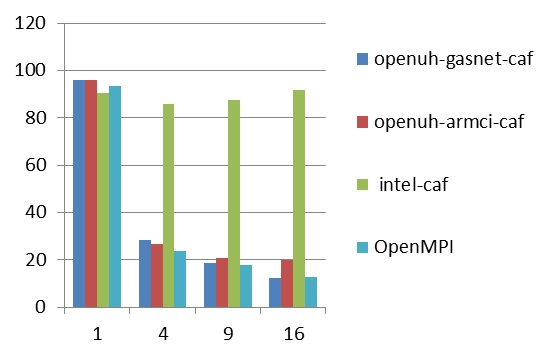
\includegraphics[width=\textwidth]{./figures/bt_A_time.jpg}
\caption{BT, CLASS=A}
\label{fig:figure1}
\end{minipage}
\hspace{0.5cm}
\begin{minipage}[b]{0.45\linewidth}
\centering
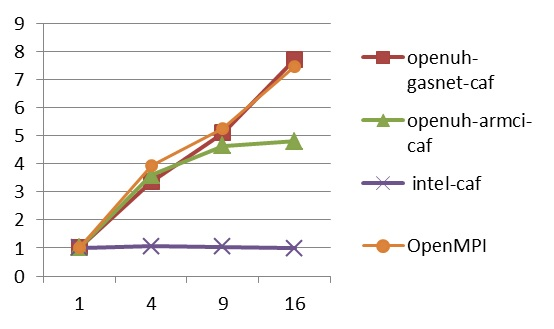
\includegraphics[width=\textwidth]{./figures/bt_A_scalability.jpg}
\caption{BT, CLASS=A}
\label{fig:figure2}
\end{minipage}
\end{figure}



\begin{figure}[ht]
\begin{minipage}[b]{0.45\linewidth}
\centering
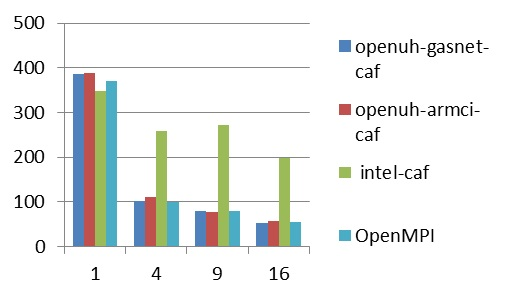
\includegraphics[width=\textwidth]{./figures/bt_B_time.jpg}
\caption{BT, CLASS=B}
\label{fig:figure1}
\end{minipage}
\hspace{0.5cm}
\begin{minipage}[b]{0.45\linewidth}
\centering
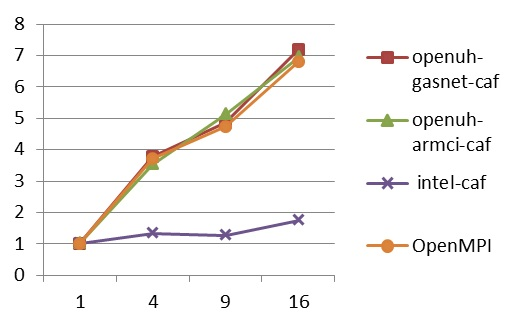
\includegraphics[width=\textwidth]{./figures/bt_B_scalability.jpg}
\caption{BT, CLASS=B}
\label{fig:figure2}
\end{minipage}
\end{figure}


\begin{figure}[ht]
\begin{minipage}[b]{0.45\linewidth}
\centering
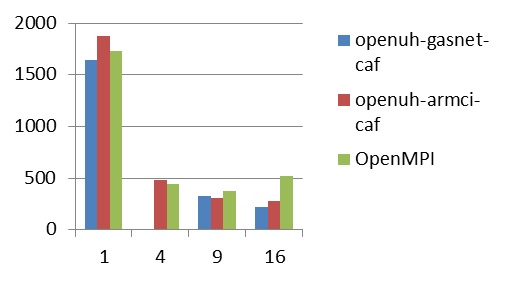
\includegraphics[width=\textwidth]{./figures/bt_C_time.jpg}
\caption{BT, CLASS=C}
\label{fig:figure1}
\end{minipage}
\hspace{0.5cm}
\begin{minipage}[b]{0.45\linewidth}
\centering
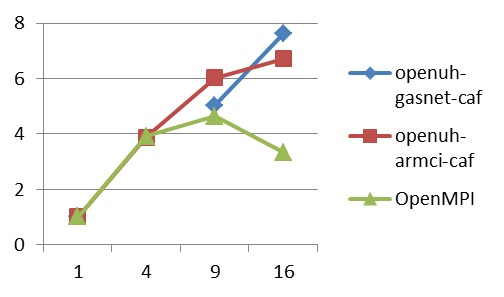
\includegraphics[width=\textwidth]{./figures/bt_C_scalability.jpg}
\caption{BT, CLASS=C}
\label{fig:figure2}
\end{minipage}
\end{figure}




%\bibliographystyle{plain}
%\bibliography{references}

\end{document}
